\documentclass[11pt]{beamer}
\usepackage{verbatim}
\usepackage{amsmath}
\usepackage{amsthm}
\usepackage{graphics}
\usepackage{multicol}
\usepackage{color}
\usepackage{stmaryrd}
\usefonttheme[onlymath]{serif}

\title{Progess Report 8}
\date{\today}
\author{Xie Li}
\begin{document}
\maketitle

\begin{frame}\frametitle{Overview of the Progress}
\begin{itemize}
\item Run several cases and find some problems.
\item Debugging of the tool.
\item Other: prepare the talk, journal paper rectify and other project.
\end{itemize}

\end{frame}


\begin{frame}\frametitle{Flowgraph of the tool}

\begin{center}
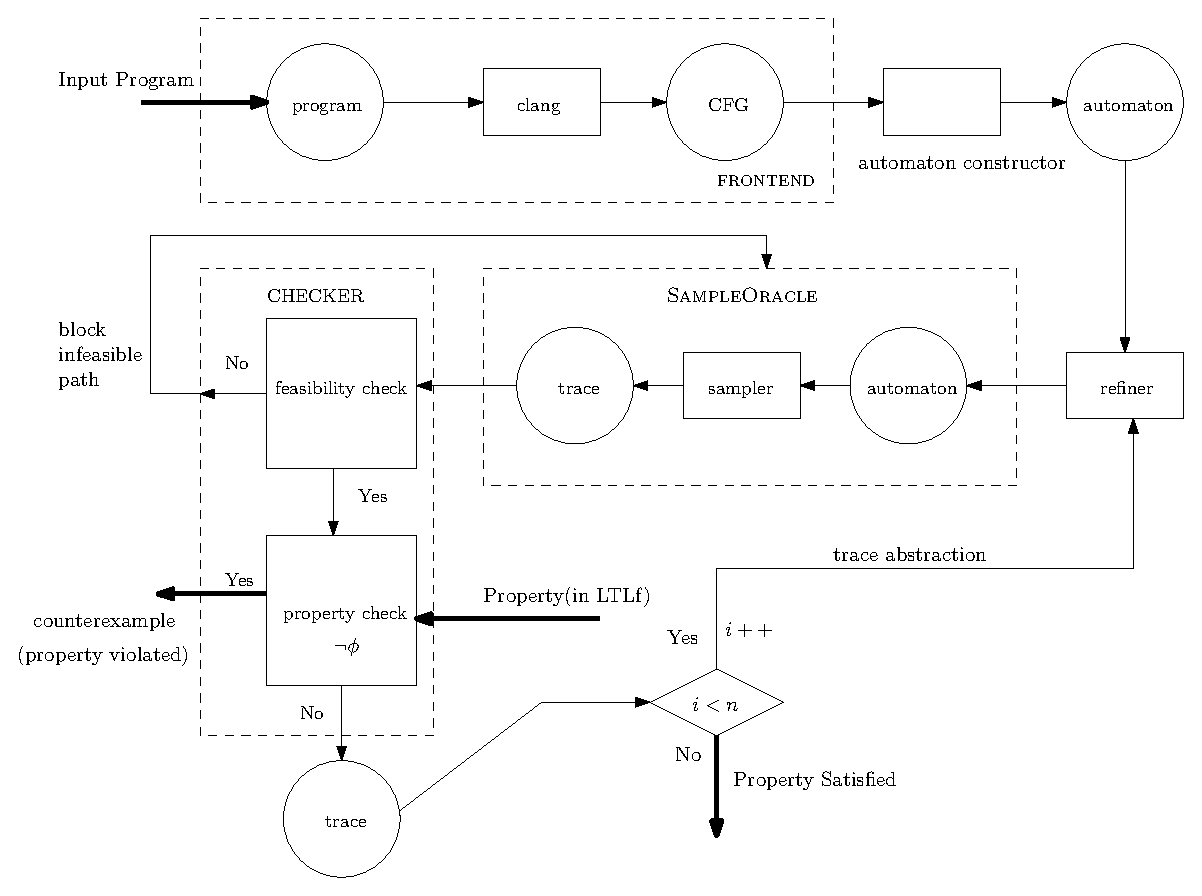
\includegraphics[scale=0.5]{dataflow.eps}
\end{center}

\end{frame}

\begin{frame}\frametitle{Current problem}
The meaningless of checking $\mathbf{G}\phi$ property. How to seperate the state?

\end{frame}

\begin{frame}\frametitle{Experiment on cases}
Handcrafted and a few cases of \textsc{SV-COMP}.

\begin{center}
\includegraphics[scale=0.4]{2nested.png}
\includegraphics[scale=.4]{test4.png}
\end{center}
\end{frame}

\begin{frame}\frametitle{Experiment on cases}
\begin{center}
\includegraphics[scale=0.4]{Bangalore.png}
\includegraphics[scale=.4]{test1.png}
\includegraphics[scale=.4]{test2.png}
\end{center}
\end{frame}

\begin{frame}\frametitle{Later work}

\begin{itemize}

\item Adapt the format of \textsc{SV-COMP}. This require some work at the frontend and a more closer look at \textsc{SV-COMP}.

\item To conduct large scale experiment, the support of the interface needs to be more precise and robust. 
\end{itemize}


\end{frame}


\end{document}